\documentclass[tikz,border=4pt]{standalone}
\usepackage[T1]{fontenc}
\usepackage{lmodern}
\usetikzlibrary{arrows.meta,positioning,fit,backgrounds,calc,shapes.geometric,decorations.pathreplacing}
\begin{document}
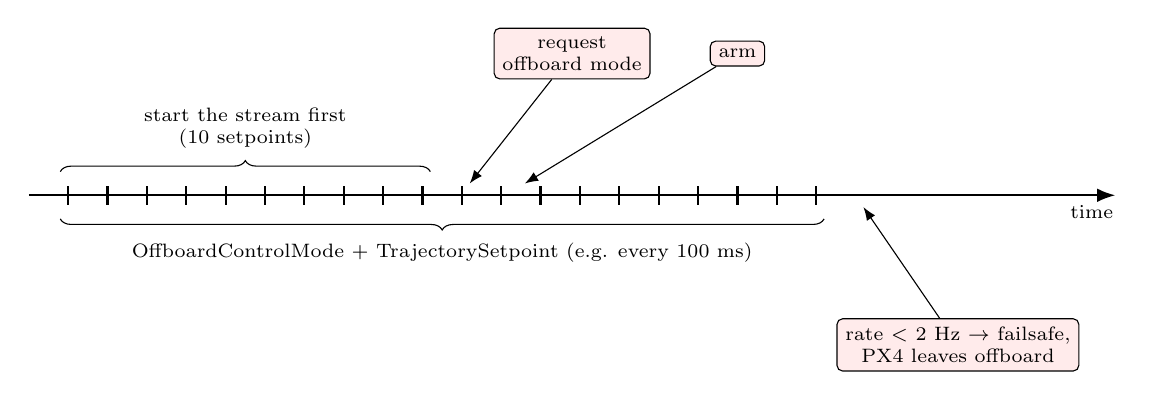
\begin{tikzpicture}[
  ev/.style={draw,rounded corners=2pt,font=\scriptsize,align=center,fill=red!8,inner sep=3pt},
  >={Latex}]
\draw[->,thick] (0,0) -- (13.8,0) node[below,font=\scriptsize,xshift=-3mm] {time};
\foreach \i in {0,...,19} \draw[thick] (0.5+0.5*\i,-0.12) -- (0.5+0.5*\i,0.12);
\draw[decorate,decoration={brace,amplitude=4pt}] (0.4,0.3) -- (5.1,0.3) node[midway,above=5pt,font=\scriptsize,align=center] {start the stream first\\(10 setpoints)};
\draw[decorate,decoration={brace,amplitude=4pt,mirror}] (0.4,-0.3) -- (10.1,-0.3) node[midway,below=5pt,font=\scriptsize] {OffboardControlMode + TrajectorySetpoint (e.g. every 100 ms)};
\draw[dashed] (10.1,0) -- (11.4,0);
\node[ev] (e1) at (6.9,1.8) {request\\offboard mode};
\node[ev] (e2) at (9.0,1.8) {arm};
\draw[->] (e1) -- (5.6,0.15);
\draw[->] (e2) -- (6.3,0.15);
\node[ev] (e3) at (11.8,-1.9) {rate $<$ 2 Hz $\rightarrow$ failsafe,\\PX4 leaves offboard};
\draw[->] (e3) -- (10.6,-0.15);
\end{tikzpicture}
\end{document}
